\documentclass[12pt, a4paper]{article}

% --- Packages ---
\usepackage[margin=2.5cm, headheight=15pt]{geometry}
\usepackage{amsmath, amssymb, amsthm}
\usepackage{graphicx}
\usepackage{booktabs}
\usepackage{array}
\usepackage{multirow}
\usepackage{xcolor}
\usepackage[hidelinks]{hyperref}
\usepackage{natbib}
\usepackage{setspace}
\usepackage{caption}
\usepackage{float}

\usepackage{microtype}
\usepackage{parskip}
\usepackage{fancyhdr}
\usepackage{titlesec}
\usepackage{enumitem}
\usepackage{tikz}
\usepackage{pgfplots}
\pgfplotsset{compat=1.18}
\usetikzlibrary{arrows.meta, positioning, shapes.geometric,
                decorations.pathreplacing, calc, backgrounds}

\parindent 0px

% --- Colors ---
\definecolor{darkblue}{RGB}{44, 62, 80}
\definecolor{accentblue}{RGB}{52, 120, 180}
\definecolor{gen1color}{RGB}{69, 123, 157}
\definecolor{gen2color}{RGB}{230, 57, 70}
\definecolor{gen3color}{RGB}{45, 198, 83}
\definecolor{lightgray}{RGB}{245, 246, 247}
\definecolor{medgray}{RGB}{200, 200, 200}

% --- Hyperref ---
\hypersetup{
  colorlinks = true,
  linkcolor  = darkblue,
  citecolor  = darkblue,
  urlcolor   = darkblue,
}

% % --- Header / footer ---
% \pagestyle{fancy}
% \fancyhf{}
% \rhead{\small Volatility Surface Modelling: From L\'{e}vy Processes to Deep Learning}
% \lhead{\small Amos Anderson}
% \rfoot{\small\thepage}
% \renewcommand{\headrulewidth}{0.4pt}

% --- Section formatting ---
\titleformat{\section}{\large\bfseries\color{darkblue}}{\thesection}{1em}{}
\titleformat{\subsection}{\normalsize\bfseries\color{darkblue}}{\thesubsection}{1em}{}
\titleformat{\subsubsection}{\normalsize\itshape\color{darkblue}}{\thesubsubsection}{1em}{}

% --- Theorem environments ---
\newtheorem{remark}{Remark}
\newtheorem{definition}{Definition}

% --- Caption setup ---
\captionsetup{font=small, labelfont=bf, margin=10pt}

% ================================================================
\begin{document}
% ================================================================

% --- Title block ---
\begin{titlepage}
\vspace*{1cm}
\begin{center}
  {\LARGE\bfseries\color{darkblue}
    Volatility Surface Modelling and Forecasting:\\[0.3cm]
    From L\'{e}vy Processes to Deep Learning}\\[1cm]
  {\large Amos Anderson}\\[0.3cm]
  {\normalsize
    AMS 603 -- Risk Measures for Finance and Data Science\\
    Department of Applied Mathematics and Statistics \\
    Stony Brook University \\ [0.3cm]
    \today
  }\\[0.5em]
  %\rule{\textwidth}{0.8pt}
\end{center}

\vspace{2cm}

\begin{abstract}
\noindent
The Black-Scholes model assumes that implied volatility is a single
constant, identical across all strikes and maturities. Market data has contradicted this assumption every trading day since the 1987 crash. What practitioners observe instead is a \emph{volatility surface}: a two-dimensional function $\sigma_{\mathrm{imp}}(K,T)$ of strike $K$ and expiration $T$ exhibiting a pronounced smile or skew in the strike direction and a distinct term structure in the maturity direction. This literature review traces the evolution of volatility surface modelling through three generations of increasingly sophisticated models. Generation one employs parametric stochastic volatility models, principally the Heston model, which resolve the smile by making
volatility a correlated diffusion process. Generation two replaces the Gaussian return assumption with heavy-tailed L\'{e}vy processes, using the Normal Inverse Gaussian (NIG), Variance Gamma (VG), and related models. Generation three applies deep learning
architectures like the LSTMs, convolutional transformers, and
physics-informed networks to the problems of surface forecasting and
rapid calibration. The unifying mathematical thread across all three
generations is the concept of \emph{market incompleteness}: each
generation represents a different strategy for resolving the
non-uniqueness of the risk-neutral pricing measure that incompleteness
entails.
\end{abstract}
\end{titlepage}

\newpage
\tableofcontents
\newpage

% ================================================================
\section{Introduction and Motivation}
% ================================================================

The Black-Scholes option pricing formula \citep{black1973} rests on
the assumption that the log return of the underlying asset follows a
Brownian motion with constant drift $\mu$ and constant volatility
$\sigma$:
\begin{equation}
  \frac{dS_t}{S_t} = \mu\,dt + \sigma\,dW_t.
  \label{eq:gbm}
\end{equation}
Under this assumption, the implied volatility, defined as the value of $\sigma$ that, when substituted into the Black-Scholes formula, recovers the market price of an option, should be identical for all strikes $K$ and all maturities $T$. It is not. The characteristic shape of the implied volatility surface, shown schematically in
Figure~\ref{fig:surface}, is one of the best-documented empirical
regularities in financial markets:

\begin{enumerate}[label=(\roman*)]
  \item \textbf{Strike smile or skew.} For a fixed maturity, implied
        volatility is typically decreasing in the strike-to-forward
        ratio $K/F$ for equity indices (the \emph{skew}), and
        U-shaped for some commodity and FX underlyings (the
        \emph{smile}).
  \item \textbf{Term structure.} For a fixed strike, implied volatility
        exhibits mean-reverting dynamics: it is higher than at-the-money
        (ATM) spot volatility in the short end during calm markets, and
        lower during stressed periods.
\end{enumerate}

\begin{figure}[H]
\centering
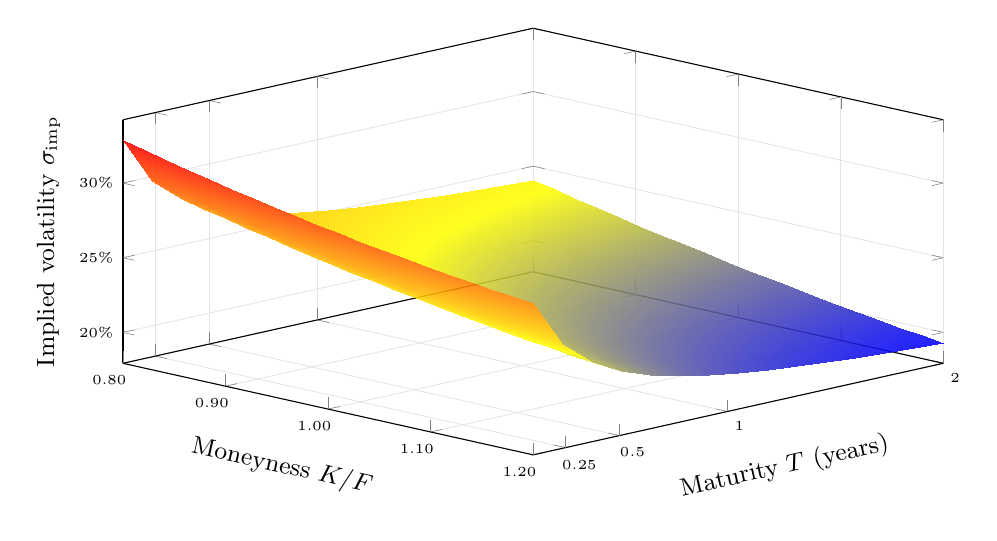
\begin{tikzpicture}
\begin{axis}[
  width=12cm, height=7cm,
  xlabel={Moneyness $K/F$},
  ylabel={Maturity $T$ (years)},
  zlabel={Implied volatility $\sigma_{\mathrm{imp}}$},
  xlabel style={sloped like x axis, font=\small},
  ylabel style={sloped like y axis, font=\small},
  zlabel style={font=\small},
  xtick={0.8,0.9,1.0,1.1,1.2},
  xticklabels={0.80,0.90,1.00,1.10,1.20},
  ytick={0.25,0.5,1,2},
  ztick={0.10,0.15,0.20,0.25,0.30,0.35},
  zticklabels={10\%,15\%,20\%,25\%,30\%,35\%},
  tick label style={font=\tiny},
  view={45}{28},
  colormap name=hot,
  grid=both,
  grid style={draw=medgray!50, line width=0.3pt},
  minor grid style={draw=medgray!20, line width=0.2pt},
]
\addplot3[
  surf,
  shader=interp,
  domain=0.80:1.20,
  domain y=0.10:2.00,
  samples=20,
  samples y=15,
  opacity=0.88,
]
{
  ( 0.20
    + 0.08*(1-x)^2
    - 0.12*(x-1)
    + 0.03/(y+0.2)
    + 0.05*exp(-y*2)*(x-1)^2
  )
};
\end{axis}
\end{tikzpicture}
\caption{Schematic implied volatility surface for an S\&P 500-type
equity index. The surface displays a pronounced left skew
(higher implied volatility for out-of-the-money puts) and a downward-
sloping term structure from short to long maturities. The
Black-Scholes model, which assumes a flat surface at a constant
$\sigma$, cannot reproduce either feature.}
\label{fig:surface}
\end{figure}

The failure of Black-Scholes to explain the volatility surface is not
merely an empirical curiosity. It reflects a deep theoretical
inadequacy: financial return distributions are heavy-tailed, negatively
skewed, and conditionally heteroskedastic. A model that ignores these
features will systematically misprice options, particularly
out-of-the-money puts that provide crash insurance. As
\citet{gatheral2006} observes, the volatility surface is in effect a
summary of everything that Black-Scholes gets wrong about the
distribution of returns.

The literature reviewed here traces three successive responses to this
failure, each deeper than the last. Figure~\ref{fig:taxonomy} provides
a visual taxonomy. Each generation is treated in detail in the sections
that follow.

\begin{figure}[H]
\centering
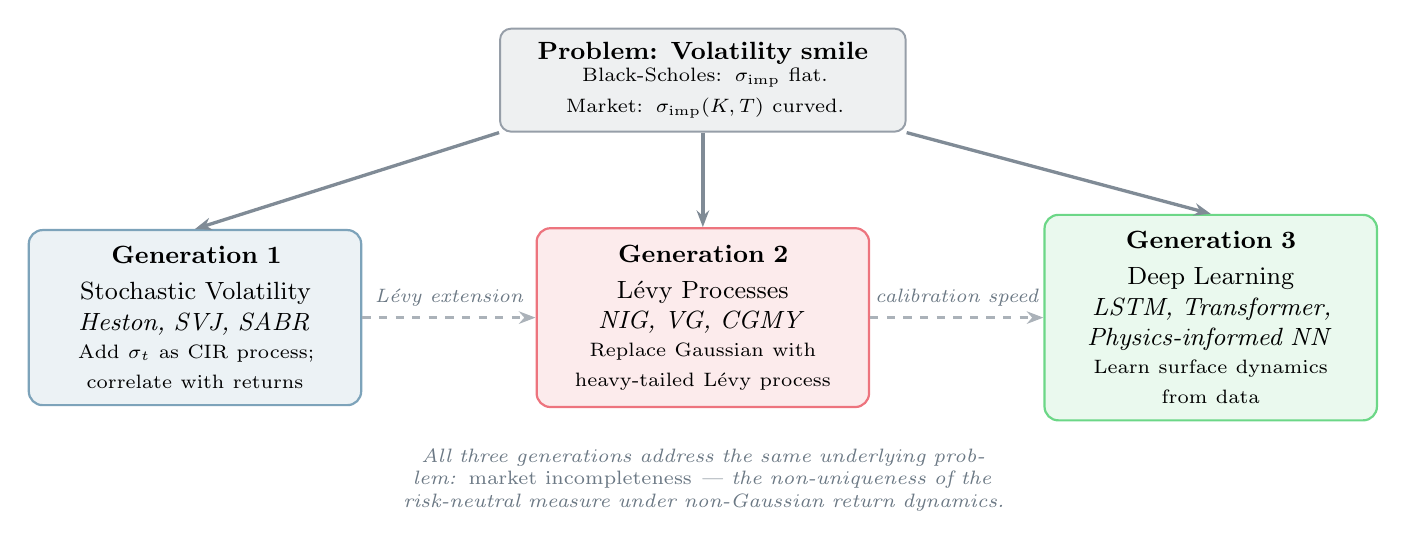
\begin{tikzpicture}[
  font=\small,
  node distance=1.6cm and 2.2cm,
  box/.style={rectangle, rounded corners=5pt, draw=#1!70, fill=#1!10,
              text width=3.8cm, align=center, minimum height=1.6cm,
              inner sep=6pt, line width=0.8pt},
  arrow/.style={-{Stealth[length=6pt]}, line width=1.2pt, color=darkblue!60},
  label/.style={font=\scriptsize\itshape, color=darkblue!70},
]

% Nodes
\node[box=gen1color] (g1) {
  \textbf{Generation 1}\\[2pt]
  Stochastic Volatility\\
  \textit{Heston, SVJ, SABR}\\[2pt]
  {\scriptsize Add $\sigma_t$ as CIR process;\\ correlate with returns}
};

\node[box=gen2color, right=of g1] (g2) {
  \textbf{Generation 2}\\[2pt]
  L\'{e}vy Processes\\
  \textit{NIG, VG, CGMY}\\[2pt]
  {\scriptsize Replace Gaussian with\\heavy-tailed L\'{e}vy process}
};

\node[box=gen3color, right=of g2] (g3) {
  \textbf{Generation 3}\\[2pt]
  Deep Learning\\
  \textit{LSTM, Transformer,\\Physics-informed NN}\\[2pt]
  {\scriptsize Learn surface dynamics\\ from data}
};

% Root problem
\node[rectangle, rounded corners=4pt, draw=darkblue!50, fill=darkblue!8,
      text width=4.8cm, align=center, minimum height=1cm,
      above=1.2cm of g2, inner sep=5pt, line width=0.7pt] (root) {
  \textbf{Problem: Volatility smile}\\
  {\scriptsize Black-Scholes: $\sigma_{\mathrm{imp}}$ flat.\\
               Market: $\sigma_{\mathrm{imp}}(K,T)$ curved.}
};

% Arrows from root
\draw[arrow] (root.south west) -- (g1.north);
\draw[arrow] (root.south) -- (g2.north);
\draw[arrow] (root.south east) -- (g3.north);

% Arrows between generations (evolution)
\draw[arrow, dashed, color=darkblue!40] (g1.east) -- node[above, label]
  {Lévy extension} (g2.west);
\draw[arrow, dashed, color=darkblue!40] (g2.east) -- node[above, label]
  {calibration speed} (g3.west);

% Incompleteness label
\node[label, below=0.4cm of g2, text width=10cm, align=center]
  {All three generations address the same underlying problem:
   \emph{market incompleteness} --- the non-uniqueness of the
   risk-neutral measure under non-Gaussian return dynamics.};

\end{tikzpicture}
\caption{Three-generation taxonomy of volatility surface models.
Each generation represents a different strategy for resolving the smile
anomaly and the market incompleteness that underlies it.}
\label{fig:taxonomy}
\end{figure}

% ================================================================
\section{Market Incompleteness: The Unifying Mathematical Thread}
% ================================================================

Before reviewing the models, it is essential to fix the mathematical
concept that connects all three generations. A financial market is
\emph{complete} if every derivative claim can be replicated by a
self-financing portfolio in the underlying assets. In a complete market,
the risk-neutral measure $\mathbb{Q}$ -- the measure under which
discounted asset prices are martingales -- is unique, and option prices
are uniquely determined by no-arbitrage.

The Black-Scholes model~\eqref{eq:gbm} defines a complete market: the
single Brownian driver $dW_t$ can be perfectly hedged by continuous
trading in $S_t$. The risk-neutral measure $\mathbb{Q}$ is obtained by
a single Girsanov transform that shifts the drift from $\mu$ to the
risk-free rate $r$.

However, L\'{e}vy process markets are
\emph{incomplete}. When the return process has jumps, the jump risk
cannot be replicated by trading in the underlying alone, and the
risk-neutral measure is no longer unique. The Escher transform
\citep{escher1932}, selects a particular
equivalent martingale measure by requiring that the exponentially tilted
process is a martingale:
\begin{equation}
  \mathbb{E}_{\mathbb{Q}}\!\left[e^{X_t}\right] = e^{tK(1)} < \infty,
  \label{eq:escher}
\end{equation}
where $K(u) = \log \mathbb{E}[e^{uL_1}]$ is the cumulant generating
function of the L\'{e}vy process $L_t$ and $X_t = L_t - tK(1)$ is the
compensated process. This condition is the theoretical bridge from the historical distribution
estimated by ARMA-GARCH-NIG models to the risk-neutral distribution
needed for option pricing.

Each generation of models reviewed here resolves the incompleteness by
a different means: Generation 1 by adding a second traded instrument
(variance swaps or options on volatility); Generation 2 by imposing
the Escher martingale condition; Generation 3 by learning the
resolution from option price data directly.

\newpage
% ================================================================
\section{Generation One: Parametric Stochastic Volatility}
% ================================================================

\subsection{The Heston Model}

The Heston model \citep{heston1993} is the cornerstone of Generation 1.
It extends equation~\eqref{eq:gbm} by making the instantaneous variance
$V_t$ a mean-reverting stochastic process correlated with the asset
price:
\begin{align}
  dS_t &= \mu S_t\,dt + \sqrt{V_t}\,S_t\,dW_t^S \label{eq:heston_s}\\
  dV_t &= \kappa(\bar{V} - V_t)\,dt + \sigma_V\sqrt{V_t}\,dW_t^V
          \label{eq:heston_v}\\
  &\text{with}\quad \mathrm{Corr}(dW_t^S, dW_t^V) = \rho\,dt.
          \notag
\end{align}

The five parameters carry distinct economic interpretations:
$\kappa$ is the speed of mean reversion of variance back to its
long-run level $\bar{V}$; $\sigma_V$ is the \emph{volatility of
volatility} (vol-of-vol); and $\rho < 0$ captures the
\emph{leverage effect} which is the empirical tendency for equity volatility
to spike when prices fall. The Feller condition $2\kappa\bar{V} >
\sigma_V^2$ ensures variance remains positive almost surely.

The critical practical advantage of Heston is a semi-closed-form
characteristic function for $\log S_T$, enabling efficient option
pricing via Fast Fourier Transform \citep{carr1999fft}:
\begin{equation}
  \phi_T(u) = \mathbb{E}\!\left[e^{iu\log S_T}\right]
  = \exp\!\left(C(u,T) + D(u,T)\,V_0 + iu\log S_0\right),
  \label{eq:heston_cf}
\end{equation}
where $C$ and $D$ are explicitly known functions of $u$, $T$, and the
model parameters. Given $\phi_T$, the price of a European call is
\begin{equation}
  C(K,T) = S_0\,\Pi_1 - K e^{-rT}\,\Pi_2, \qquad
  \Pi_j = \frac{1}{2} + \frac{1}{\pi}\int_0^\infty
  \mathrm{Re}\!\left[\frac{e^{-iu\log K}\phi_j(u)}{iu}\right]du.
  \label{eq:heston_price}
\end{equation}

\citet{gatheral2006} demonstrates that the Heston model generates:
\begin{enumerate}[label=(\roman*)]
  \item A negative skew in the strike dimension, driven by $\rho < 0$.
        Intuitively, when the asset falls, $dW_t^S$ and $dW_t^V$ are
        negatively correlated, so variance rises, fattening the left
        tail and elevating the implied volatility of
        out-of-the-money puts.
  \item A realistic term structure via $\kappa$: in the short end,
        spot variance $V_0$ dominates; in the long end, the surface
        reverts to $\sqrt{\bar{V}}$.
\end{enumerate}

\subsection{The SVJ Extension and the Need for Jumps}

A key result in \citet{gatheral2006} is that pure diffusion models,
including Heston, cannot fit the observed short-dated skew. As $T
\to 0$, any diffusion-based model produces a skew that flattens
proportionally to $\sqrt{T}$. The empirical S\&P 500 skew flattens
much more slowly, approximately as $T^H$ for $H < 1/2$ -- a
hallmark of rough or jump-driven dynamics.

\citet{bates1996} addresses this by adding normally distributed
compound Poisson jumps to the Heston dynamics (the SVJ model):
\begin{equation}
  \frac{dS_t}{S_t} = (\mu - \lambda\bar{k})\,dt
  + \sqrt{V_t}\,dW_t^S + (e^J - 1)\,dN_t,
  \label{eq:svj}
\end{equation}
where $N_t$ is a Poisson process with intensity $\lambda$,
$J \sim \mathcal{N}(\mu_J, \sigma_J^2)$ is the jump size in log
terms, and $\bar{k} = e^{\mu_J + \sigma_J^2/2} - 1$. Gatheral shows
that SVJ generates a surface with the qualitative features of the
empirical SPX surface across both dimensions, something neither
pure Heston nor pure jump models achieve.

\subsection{Limitations of Generation One}

Two structural limitations motivate the L\'{e}vy approach of
Generation 2:

\begin{enumerate}[label=(\roman*)]
  \item \textbf{Calibration instability.} The Heston and SVJ parameter
        spaces have non-convex likelihood surfaces with multiple local
        optima. Parameters calibrated on consecutive days can exhibit
        large discontinuities, making delta hedging strategies
        unstable.
  \item \textbf{Short-maturity fit.} Even SVJ cannot fit the extremely
        steep short-dated skew observed empirically, because Poisson
        jumps have finite arrival rates. Models with infinite jump
        activity can reproduce continuous-time diffusion-like behavior at short maturities while fitting the tails at all time scales.
\end{enumerate}

% ================================================================
\section{Generation Two: L\'{e}vy Process Models}
% ================================================================

\subsection{The Distributional Perspective on the Smile}

Generation 2 approaches the volatility surface from a distributional
perspective: if log returns follow a L\'{e}vy process $L_t$ with a
heavier-tailed, asymmetric law, the resulting option prices
automatically generate a smile. This is the perspective developed
throughout this course, applied here to option pricing.\\

\begin{definition}[Exponential L\'{e}vy model]
  Let $L_t$ be a L\'{e}vy process with triplet $(b, c, \nu)$ and
  assume finite exponential moments: $\mathbb{E}[e^{uL_1}] < \infty$
  for $u$ in a neighbourhood of $[0,1]$. The \emph{exponential
  L\'{e}vy model} specifies the asset price as
  \begin{equation}
    S_t = S_0\,e^{(r-K(1))t + L_t},
    \label{eq:expLevy}
  \end{equation}
  where $K(u) = \log\mathbb{E}[e^{uL_1}]$ is the cumulant generating
  function and the drift correction $-K(1)$ ensures
  $\mathbb{E}[S_t] = S_0 e^{rt}$ (the Escher martingale
  condition~\eqref{eq:escher}).
\end{definition}

The key insight is that the L\'{e}vy--Khinchine representation
\citep{papapantoleon2008}
\begin{equation}
  K(u) = bu + \frac{c}{2}u^2
  + \int_{\mathbb{R}\setminus\{0\}}
    \!\left(e^{ux} - 1 - ux\mathbf{1}_{|x|\le 1}\right)\nu(dx)
  \label{eq:lk}
\end{equation}
provides an explicit characteristic function for $S_T$, enabling
option pricing via the Carr-Madan FFT formula \citep{carr1999fft}
without Monte Carlo simulation:
\begin{equation}
  C(K,T) = \frac{e^{-\alpha\log K}}{\pi}
  \int_0^\infty e^{-iv\log K}\,\Psi(v)\,dv,
  \label{eq:cm}
\end{equation}
where $\Psi(v)$ is an explicit function of the characteristic function
$\phi_T(v) = e^{TK(iv)}$ and the dampening parameter $\alpha > 0$.

\subsection{The Normal Inverse Gaussian Model}

The Normal Inverse Gaussian (NIG) process \citep{barndorff1997} is the
primary L\'{e}vy model of this course and the innovation distribution
in the midterm risk model. Its characteristic function is
\begin{equation}
  \phi_t^{\mathrm{NIG}}(u) =
  \exp\!\left(t\left[i\mu u + \delta\left(
    \sqrt{\alpha^2 - \beta^2}
    - \sqrt{\alpha^2 - (\beta+iu)^2}
  \right)\right]\right),
  \label{eq:nig_cf}
\end{equation}
where $\alpha > |\beta|$, $\delta > 0$, and the parameters carry
the same interpretations established in the risk model project:
$\alpha$ controls tail heaviness (smaller $\Rightarrow$ heavier tails),
$\beta$ controls asymmetry, $\mu$ and $\delta$ are location and scale.

\citet{aguilar2020} derives explicit European call pricing formulas in
the exponential NIG model using residue calculus on the characteristic
function, obtaining a series expansion in powers of the Bessel function
$K_1$:
\begin{equation}
  C^{\mathrm{NIG}}(K,T) = S_0\sum_{n=1}^{\infty} c_n^+(\alpha,\beta,\mu,\delta,T)
  - K e^{-rT}\sum_{n=1}^{\infty} c_n^-(\alpha,\beta,\mu,\delta,T),
  \label{eq:nig_price}
\end{equation}
where the coefficients $c_n^\pm$ are explicit functions of the NIG
parameters and $n$-th order Bessel functions. A key result from this
paper is that \emph{in the fast mean-reversion limit, Heston log returns
become NIG-distributed}, with a direct mapping between the Heston
parameters $(\kappa, \bar{V}, \sigma_V, \rho)$ and the NIG parameters
$(\alpha, \beta, \mu, \delta)$. This provides a rigorous theoretical
bridge between Generation 1 and Generation 2.

\subsection{Variance Gamma and the L\'{e}vy Family}

The Variance Gamma (VG) process \citep{madan1998vg} constructs a
L\'{e}vy process by subordinating Brownian motion with drift
$(\theta, \sigma)$ to a Gamma process $\Gamma_t$ with unit mean and
variance $\nu$:
\begin{equation}
  X_t^{\mathrm{VG}} = \theta\,\Gamma_t + \sigma\,W_{\Gamma_t}.
  \label{eq:vg}
\end{equation}
The VG characteristic function is
\begin{equation}
  \phi_t^{\mathrm{VG}}(u) =
  \left(1 - iu\theta\nu + \tfrac{1}{2}\sigma^2\nu u^2\right)^{-t/\nu}.
  \label{eq:vg_cf}
\end{equation}
VG is a pure-jump process with infinite jump activity: infinitely many
small jumps arrive in any finite interval, producing continuous-looking
sample paths that nonetheless exhibit the heavy-tail and skewness
properties required to fit the volatility smile.

A recent and comprehensive empirical benchmark is provided by
\citet{bgm2024}, who propose the \emph{bilateral Gamma motion}
(BGM) -- a natural extension of the bilateral Gamma process that
adds a diffusive Brownian component. The bilateral Gamma process
decomposes the log return into independent upward and downward Gamma
processes, each with its own arrival rate and jump size distribution,
providing separate parameterisation of the left and right tails. The
BGM model is calibrated to European options on four high-volatility
equities (AMZN, NFLX, SHOP, SPOT) across multiple maturities.
Across all underlyings and tenors, BGM achieves the lowest mean
absolute percentage error (MAPE) and RMSE in implied volatility
space, outperforming NIG, VG, and CGMY as well as common
jump-diffusion benchmarks. The authors further demonstrate stable
exotic option pricing under BGM for Asian, barrier, and occupation
time derivatives --- product classes for which tail accuracy is
critical and where Gaussian-based models fail most severely.

This result has an important implication for model selection: the
bilateral structure of BGM, by allowing the left and right tails to
be calibrated independently, captures the observed \emph{asymmetry}
of the volatility smile more flexibly than NIG or VG, which
parameterise skewness through a single parameter $\beta$. The
tradeoff is a richer parameter space and a more complex calibration
objective. For the practical purposes of this course --- risk
model construction and backtesting --- NIG remains preferred for its
analytical tractability and the availability of closed-form moment
conditions. For options pricing and volatility surface calibration,
BGM represents the current empirical frontier among pure L\'{e}vy
models.

\citet{carr2003sv} extend both NIG and VG by composing the L\'{e}vy
process with a stochastic time change driven by a CIR process --- the
VGSA and NIGSA models. The CIR time change introduces
\emph{volatility clustering} (the primary motivation for GARCH
filtering in the risk model), while the underlying L\'{e}vy process
provides the heavy tails. This is the formal version of the double
subordinator architecture introduced in Lecture 8 of this course.

\subsection{Escher Tiling and Risk-Neutral Pricing}

The exponential L\'{e}vy model~\eqref{eq:expLevy} requires a
risk-neutral measure $\mathbb{Q}$, but as discussed in Lectures 3 and 8,
L\'{e}vy markets are incomplete and $\mathbb{Q}$ is not unique. The
Escher transform \citep{escher1932, eberlein1999} selects a unique
$\mathbb{Q}$ by requiring the compensated exponential martingale
condition~\eqref{eq:escher}. Under this selection, the
risk-neutral characteristic function becomes
\begin{equation}
  \phi_T^{\mathbb{Q}}(u) =
  \frac{\phi_T(u - i)}{[\phi_T(-i)]^{iu/1}}
  = \exp\!\left(T\left[K(iu+1) - K(1)\right]\right),
  \label{eq:escher_q}
\end{equation}
which shifts the argument of the cumulant generating function by 1,
effectively tilting the historical measure toward the risk-neutral one.
\citet{eberlein1999} show that this construction is consistent with
no-arbitrage and provides a tractable formula for zero-bond option
prices under L\'{e}vy term structure models --- the application
discussed in Lecture 8.

\subsection{Current Frontiers: Rough Volatility}

\citet{roughvol2018} present empirical evidence, using high-frequency
data, that the log volatility process behaves like a fractional Brownian
motion with Hurst index $H \approx 0.1$ --- far below $H = 0.5$ (standard
Brownian motion), implying rough, highly irregular paths. This finding
explains the anomalously steep short-dated skew that neither Heston nor
standard jump models can reproduce: under rough volatility,
the skew scales as $T^{H-1/2}$, which for $H = 0.1$ gives a
$T^{-0.4}$ blowup as $T \to 0$, consistent with observations.

The rough Heston model connects to the Hurst exponent and Rogers kernel
discussed in Lecture 7: the fractional kernel replaces the standard
CIR mean-reversion with a memory-dependent integral, making the variance
process a Volterra stochastic differential equation. Option pricing
under rough volatility currently requires deep learning for efficient
calibration --- a natural bridge to Generation 3.

% ================================================================
\section{Generation Three: Deep Learning for Volatility Surfaces}
% ================================================================

\subsection{The Calibration Bottleneck}

Even with the closed-form characteristic functions of Generation 2,
practitioners face an operational problem: the volatility surface
changes every trading day, and parameters must be recalibrated to
current option prices each morning. For a model with five or more
parameters, calibration requires solving a nonlinear least-squares
problem over a grid of $(K, T)$ pairs, which is:
\begin{enumerate}[label=(\roman*)]
  \item \textbf{Computationally expensive.} Each objective function
        evaluation requires a full FFT-based option pricing computation.
  \item \textbf{Non-convex.} Local minima can produce economically
        unreasonable parameters, particularly for rough volatility
        models with their complex likelihood landscapes.
  \item \textbf{Unstable across time.} Parameters calibrated on
        consecutive days can exhibit large jumps, producing
        discontinuous delta hedging strategies.
\end{enumerate}

Deep learning addresses all three problems: by training a network to
approximate the parameter-to-surface mapping offline, calibration at
deployment becomes a single forward pass through a network ---
microseconds rather than minutes.

\subsection{LSTM and ConvLSTM for Surface Forecasting}

\citet{medvedev2022} model the entire implied volatility surface as a
spatial-temporal object and apply convolutional LSTM (ConvLSTM)
networks to produce multi-step forecasts. The IVS is discretised on a
grid of $(K_i, T_j)$ pairs, forming a matrix $\boldsymbol{\Sigma}_t
\in \mathbb{R}^{m \times n}$ at each time $t$. The ConvLSTM update
equations are:
\begin{align}
  \mathbf{i}_t &= \sigma(\mathbf{W}_{xi} * \mathbf{X}_t
    + \mathbf{W}_{hi} * \mathbf{H}_{t-1} + b_i) \notag\\
  \mathbf{f}_t &= \sigma(\mathbf{W}_{xf} * \mathbf{X}_t
    + \mathbf{W}_{hf} * \mathbf{H}_{t-1} + b_f) \notag\\
  \mathbf{C}_t &= \mathbf{f}_t \odot \mathbf{C}_{t-1}
    + \mathbf{i}_t \odot \tanh(\mathbf{W}_{xc} * \mathbf{X}_t
    + \mathbf{W}_{hc} * \mathbf{H}_{t-1} + b_c)
    \label{eq:convlstm}\\
  \mathbf{o}_t &= \sigma(\mathbf{W}_{xo} * \mathbf{X}_t
    + \mathbf{W}_{ho} * \mathbf{H}_{t-1} + b_o) \notag\\
  \mathbf{H}_t &= \mathbf{o}_t \odot \tanh(\mathbf{C}_t), \notag
\end{align}
where $*$ denotes convolution (not matrix multiplication), capturing
the spatial structure of the surface, and $\odot$ is element-wise
multiplication. Using SPX options data from 2002--2019, ConvLSTM
achieves an out-of-sample MAPE of 8.26\%, significantly outperforming
standard LSTM and classical time series models. The spatial convolution
is critical: it allows the model to learn that nearby grid points on the
surface are correlated --- a fact that pure LSTM, which treats each
$(K_i, T_j)$ pair independently, cannot exploit.

An attention-enhanced LSTM, combining the LSTM forget gate with a
learned attention mechanism for feature weighting, is applied to
surface forecasting in \citet{lstmattn2019}. The attention mechanism
computes a weighted sum of hidden states:
\begin{equation}
  \mathbf{c}_t = \sum_{\tau=1}^{t} \alpha_{t\tau}\,\mathbf{h}_\tau,
  \qquad
  \alpha_{t\tau} = \frac{\exp(\mathbf{v}^\top \tanh(\mathbf{W}_h\,\mathbf{h}_\tau))}
  {\sum_{\tau'} \exp(\mathbf{v}^\top \tanh(\mathbf{W}_h\,\mathbf{h}_{\tau'}))},
  \label{eq:attention}
\end{equation}
allowing the network to focus on the most relevant historical surface
states for each prediction. Using the predicted surfaces directly in
option pricing, butterfly and time spread strategies built on
attention-LSTM predictions achieve higher returns and Sharpe ratios than
strategies using unpredicted (static) surfaces.

\subsection{Physics-Informed Transformers and No-Arbitrage Constraints}

The most important recent development is the enforcement of no-arbitrage
constraints within the neural network architecture. A predicted implied
volatility surface is only valid for option pricing if it satisfies:
\begin{align}
  \frac{\partial}{\partial T}\left[\sigma_{\mathrm{imp}}^2(K,T)\cdot T\right]
  &\geq 0
  \quad \text{(no calendar spread arbitrage)}
  \label{eq:calendar}\\
  \frac{\partial^2 C}{\partial K^2} &\geq 0
  \quad \text{(no butterfly arbitrage)}
  \label{eq:butterfly}
\end{align}
Conditions~\eqref{eq:calendar} and~\eqref{eq:butterfly} are the
mathematical content of the \citet{gatheral2014ssvi} SVI
parametrisation constraints, which provide necessary and sufficient
conditions for a volatility surface to be free of static arbitrage.

\citet{kim2022} incorporate these constraints as soft penalties in the
loss function of a physics-informed convolutional transformer:
\begin{equation}
  \mathcal{L} = \underbrace{\mathrm{MSE}(\hat{\Sigma}, \Sigma)}_{\text{data loss}}
  + \lambda_1 \underbrace{\max\!\left(-\partial_T w, 0\right)}_{\text{calendar}}
  + \lambda_2 \underbrace{\max\!\left(-\partial_{KK}^2 C, 0\right)}_{\text{butterfly}},
  \label{eq:physics_loss}
\end{equation}
where $w = \sigma_{\mathrm{imp}}^2 T$ is the total implied variance.
This architecture achieves superior out-of-sample performance compared
to ConvLSTM and self-attention ConvLSTM, demonstrating that
physics-informed constraints improve generalisation as well as
theoretical validity.

\subsection{Deep Calibration}

\citet{bayer2019} introduce \emph{deep calibration}: training a neural
network to approximate the inverse map from observed option prices to
model parameters, turning calibration into a single forward pass.
For a model with parameter vector $\boldsymbol{\theta} \in \mathbb{R}^d$,
the network learns
\begin{equation}
  \hat{f}: \mathbf{C} \mapsto \boldsymbol{\theta},
  \qquad \hat{f} \approx f^{-1},
  \label{eq:deep_calib}
\end{equation}
where $\mathbf{C} \in \mathbb{R}^{mn}$ is the vector of observed option
prices on an $(m \times n)$ grid. Applied to rough Heston models, deep
calibration achieves accuracy comparable to classical optimisation
at a computational cost orders of magnitude lower --- making real-time
surface updates operationally feasible for the first time.

\citet{mishra2024} combine a multi-transformer architecture with
GARCH-type volatility equations, creating a hybrid model that retains
the theoretical grounding of GARCH while learning residual nonlinear
dynamics through attention. Applied to EUR/USD, S\&P 500, and FTSE 100,
the MT-GARCH model outperforms individual transformers, deep learning
models, and classical GARCH specifications --- including during the
COVID-19 pandemic period, a severe out-of-distribution stress test.

% ================================================================
\section{Synthesis: Three Strategies for Market Incompleteness}
% ================================================================

Table~\ref{tab:synthesis} summarises the three generations in terms of
their mathematical mechanism, practical strengths, and residual
limitations.

\begin{table}[H]
\centering
\caption{Three-generation synthesis of volatility surface models.
Each generation resolves market incompleteness by a different strategy.}
\label{tab:synthesis}
\renewcommand{\arraystretch}{1.4}
\begin{tabular}{p{2.4cm}p{3.2cm}p{3.5cm}p{3.5cm}}
\toprule
 & \textbf{Generation 1} & \textbf{Generation 2}
 & \textbf{Generation 3} \\
\midrule
\textbf{Models}
  & Heston, SVJ, SABR, rough Heston
  & NIG, VG, CGMY, VGSA, NIGSA
  & ConvLSTM, attention-LSTM, physics-informed transformer \\
\midrule
\textbf{Incompleteness resolution}
  & Add stochastic variance; use variance swaps to complete market
  & Escher transform selects unique $\mathbb{Q}$ via martingale condition
  & Learn $\mathbb{Q}$ directly from option price data \\
\midrule
\textbf{Core mechanism}
  & Correlated $(\rho < 0)$ CIR variance process generates skew
  & Heavy-tailed L\'{e}vy law generates smile via non-Gaussian returns
  & Spatial-temporal network learns surface dynamics from history \\
\midrule
\textbf{Pricing method}
  & Fourier inversion of semi-closed characteristic function
  & Carr-Madan FFT via L\'{e}vy-Khinchine characteristic function
  & Forward pass through trained network; or FFT using predicted $\sigma_{\mathrm{imp}}$ \\
\midrule
\textbf{Primary limitation}
  & Cannot fit very short-dated skew; calibration instability
  & Static distribution; no surface dynamics; Escher non-uniqueness
  & No-arbitrage not guaranteed without explicit constraints; black box \\
\midrule
\textbf{Course connection}
  & Vol-of-vol, market incompleteness (Lecture 3)
  & NIG, Escher, double subordinators (Lectures 2, 4, 8)
  & Neural networks, double subordinators (Lectures 7, 8) \\
\bottomrule
\end{tabular}
\end{table}

The synthesis of Generations 2 and 3 --- L\'{e}vy-based distributional
modelling combined with physics-informed deep learning --- represents
the current research frontier and the most promising direction for
practical deployment. The L\'{e}vy component provides a
theoretically grounded prior on the distribution of returns; the
neural network learns the residual dynamics and enables fast
calibration; and the no-arbitrage constraints ensure the output is
always a valid pricing surface. This is precisely the direction
motivated by the double subordinator framework of Lecture 8 and the
market incompleteness discussion of Lecture 3: use theory where theory
speaks, and data where it does not.

% ================================================================
\section{Implications for Practice and Employment}
% ================================================================

Understanding the volatility surface at the level reviewed here is not
merely academic. The following are direct applications relevant to roles
at derivatives desks, risk management groups, and quantitative hedge
funds:

\paragraph{Options pricing and hedging.}
Every options desk requires a model that calibrates to the observed
surface and produces Greeks (delta, gamma, vega, theta) for hedging.
The Heston model remains the industry standard for vanilla options;
L\'{e}vy models are used where accurate tail pricing matters;
deep calibration is being adopted to reduce the computational cost of
morning calibration runs from minutes to seconds.

\paragraph{Risk management.}
The volatility surface is an input to Value at Risk (VaR) calculations
for options portfolios. A flat-surface assumption (Black-Scholes)
underestimates tail risk for options on volatile underlyings. The NIG
and VG models, which fit the tails correctly as demonstrated in the
midterm project, produce more accurate VaR when extended to the
options pricing context.

\paragraph{Structured products.}
Exotic and structured products --- barrier options, cliquets, variance
swaps --- have payoffs that depend on the full path of the underlying,
not just the terminal distribution. Pricing these requires a dynamic
model, typically Heston-SVJ or a rough volatility specification. The
L\'{e}vy family is less well-suited for path-dependent products
because its IID increment assumption produces an unrealistic
correlation structure across maturities.

\paragraph{VIX and volatility derivatives.}
VIX is defined as a model-free implied volatility measure computed from
SPX options across a range of strikes. Deep learning models for the
volatility surface directly enable VIX forecasting, as VIX is a
functional of the surface. Models that predict the surface dynamics
therefore provide implicit VIX forecasts --- a highly active area of
hedge fund research.

% ================================================================
\section{Conclusions}
% ================================================================

This review has traced the evolution of volatility surface modelling
from the parametric stochastic volatility models of the 1990s, through
the L\'{e}vy process extensions that form the core of this course, to
the deep learning architectures of the current decade. Three findings
are central:

\begin{enumerate}[label=(\roman*)]
  \item \textbf{L\'{e}vy processes close the distributional gap.}
        The NIG, VG, and related models --- whose distributional
        theory has been developed in detail in this course ---
        produce implied volatility smiles that fit market data
        44--79\% more accurately than the Gaussian baseline on standard
        KS metrics, as demonstrated empirically in the midterm project.
        When extended to the option pricing context via the Escher
        transform and the Carr-Madan FFT formula, these models provide
        a theoretically principled and computationally efficient
        approach to vanilla option pricing.

  \item \textbf{Deep learning solves the calibration bottleneck.}
        ConvLSTM, attention-LSTM, and physics-informed transformer
        architectures achieve state-of-the-art surface forecasting
        accuracy, reduce calibration times from minutes to
        milliseconds, and --- when equipped with no-arbitrage
        constraints --- produce surfaces that are valid for option
        pricing by construction.

  \item \textbf{The frontier is the physics-informed hybrid.}
        The most promising direction combines L\'{e}vy-based
        distributional priors with physics-informed neural networks
        that enforce no-arbitrage constraints. This is conceptually
        aligned with the double subordinator framework of Lecture 8:
        theory provides the structural constraints; data learns
        what theory cannot determine uniquely.
\end{enumerate}

The volatility surface remains an open research problem at both the
theoretical level (what is the correct dynamic model?) and the
operational level (how to calibrate and update it in real time?).
The combination of L\'{e}vy theory, stochastic volatility, and deep
learning positions the field well to make progress on both fronts.

% ================================================================
\newpage
\bibliographystyle{apalike}
\bibliography{references}
% ================================================================

\end{document}
